% Commented out: 
% \addbibresource
% \includepdf

\documentclass[12pt,letterpaper,english,bibliography=totocnumbered, abstract=on]{scrartcl}

\usepackage{indentfirst}
\usepackage[titletoc]{appendix}
\usepackage{fullpage}
%\usepackage{subfiles}
\usepackage[T1]{fontenc}
\usepackage[utf8]{inputenc}
\usepackage{color}
%\usepackage{babel}
\usepackage{verbatim}
\usepackage[unicode=true,pdfusetitle,
bookmarks=true,bookmarksnumbered=false,bookmarksopen=false,
breaklinks=true,pdfborder={0 0 0},pdfborderstyle={},backref=false,colorlinks=true]
{hyperref}
\hypersetup{linkcolor=blue,citecolor=blue,urlcolor=blue}

\usepackage{booktabs}
\usepackage{multirow}
\usepackage{adjustbox}
\usepackage{threeparttable}
\usepackage[table]{xcolor}
\usepackage{csquotes}
\usepackage{soul} % for hiliting text: \hl

\usepackage[utf8]{inputenc}
\usepackage[english]{babel}
%\usepackage{biblatex}
%\addbibresource{sample.bib}



%\usepackage[backend=biber, maxbibnames=99, dashed=false]{biblatex}
\usepackage[backend=biber, maxbibnames=99]{biblatex}
\DeclareNameAlias{author}{family-given}
%\setlength\bibitemsep{2\itemsep}
\addbibresource{blr.bib}
%\addbibresource{CRB.bib}

\usepackage{pdfpages}
\usepackage{float} % Allows use of H to place floats

\usepackage{pgfgantt}

\usepackage{framed}

\usepackage{longtable}

% Prevent page breaks within paragraphs
% https://tex.stackexchange.com/questions/21983/how-to-avoid-page-breaks-inside-paragraphs
\widowpenalties 1 10000

\begin{document}

\titlehead{Final Report: McIntire-Stennis Project XXXX}

\title{Building a Terrestrial Biodiversity Inventory for Guam}

\author{Aubrey Moore PhD}

\maketitle
%\footnote{\url{https://github.com/aubreymoore/2020-FS-CRB-biocontrol-project/blob/master/combined-proposal.pdf}}
\newpage
\tableofcontents

\pagebreak

\section{Introduction}

% TODO: \usepackage{graphicx} required
\begin{figure}
	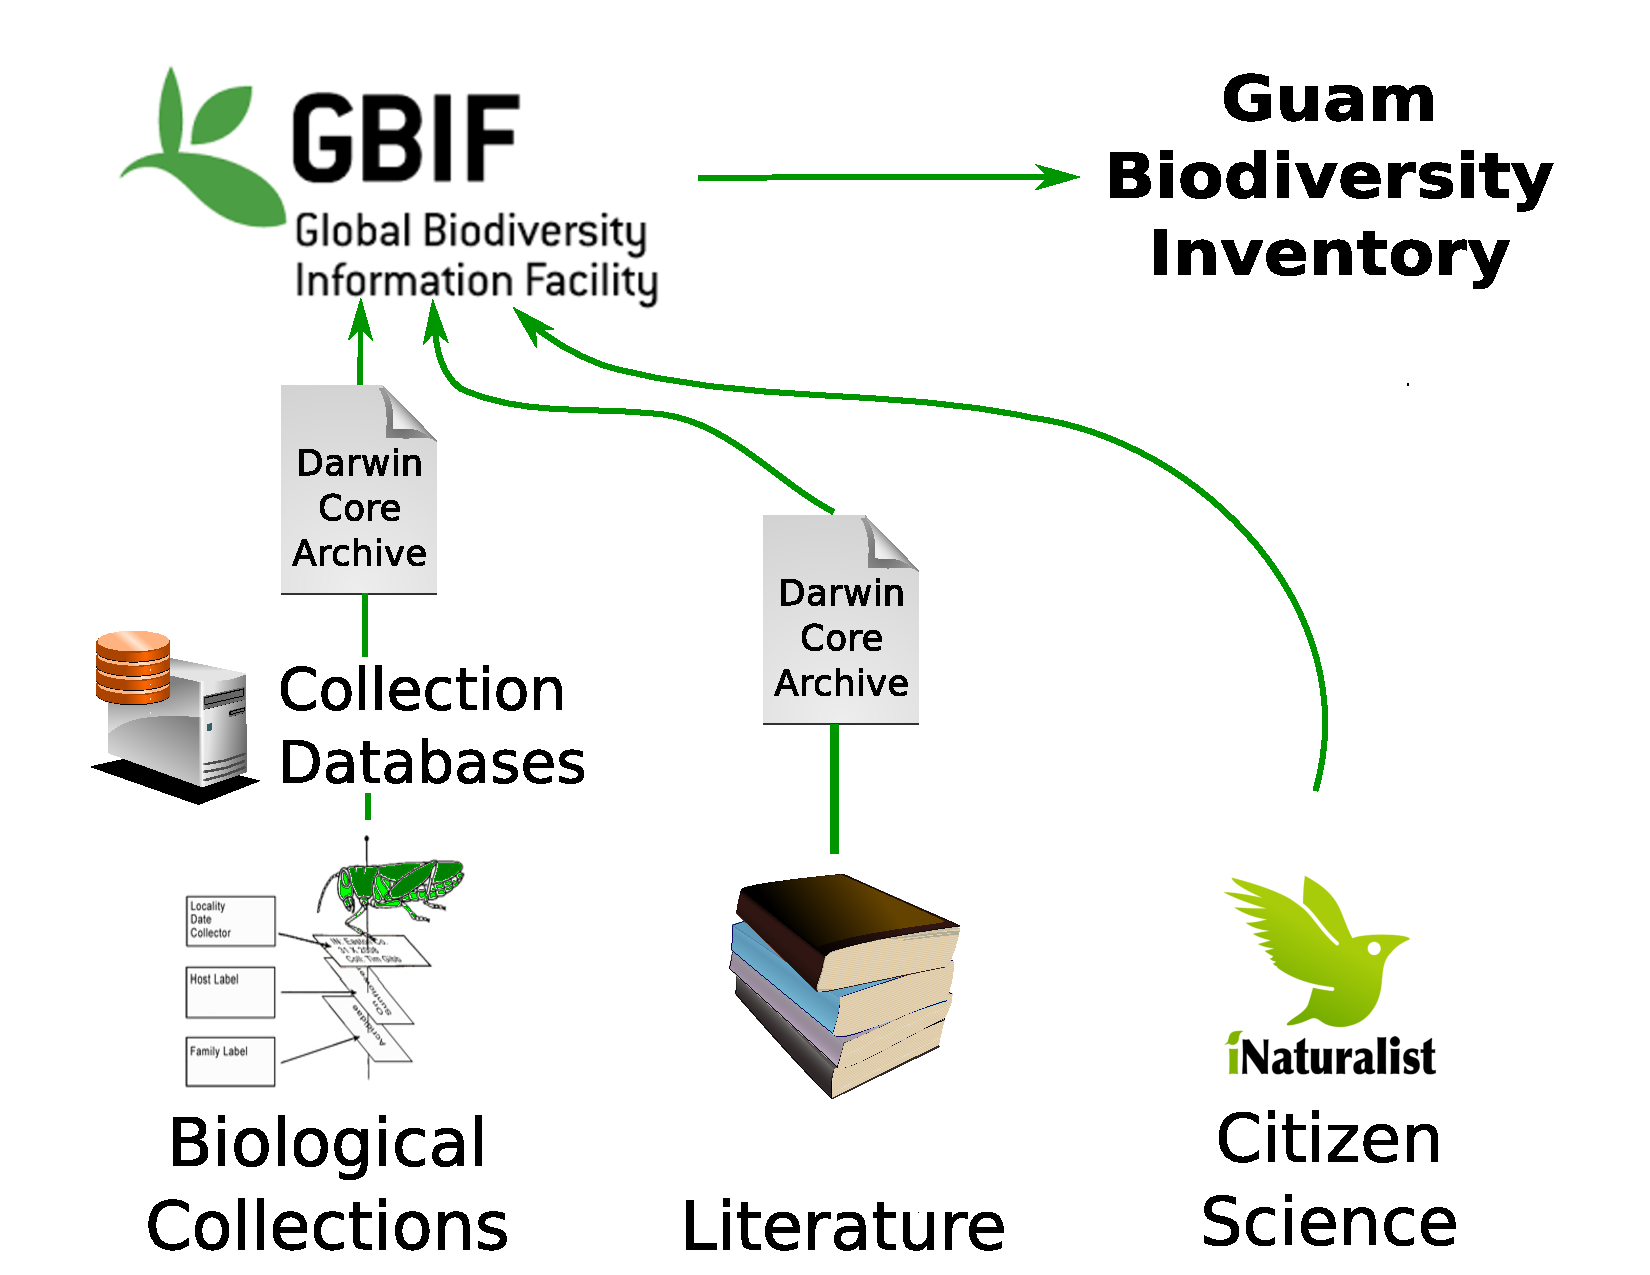
\includegraphics[width=\linewidth]{images/diag1}
	\caption{caption goes here}
	\label{fig:diag1}
\end{figure}


\pagebreak
\section{Data from the University of Guam Insect Collection}
\subsection{Acknowledgments}


\pagebreak
\section{Data from Insects of Guam Publications}

\nocite{*}
\printbibliography[heading=none]

\subsection{Acknowledgments}


\pagebreak
\section{Data from iNaturalist}
\subsection{Acknowledgments}


\pagebreak
\section{Guam Biodiversity Information from the GBIF}

% TODO: \usepackage{graphicx} required
\begin{figure}[H]
	\centering
	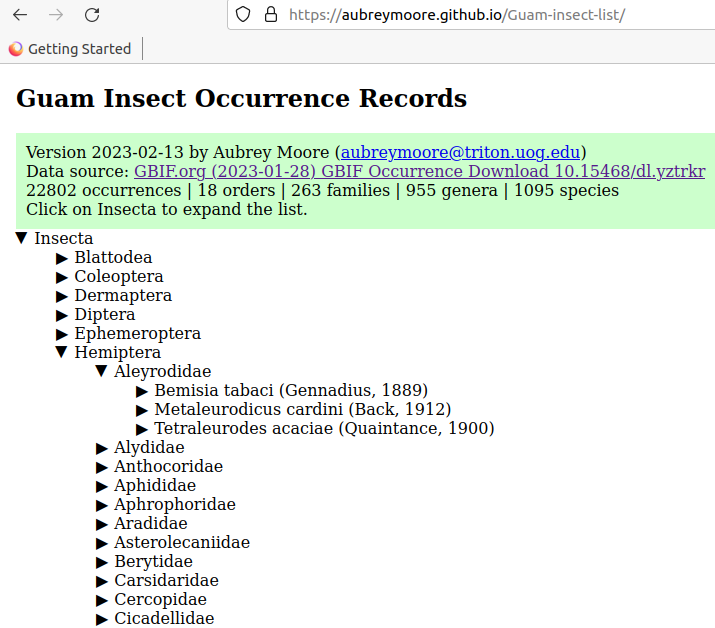
\includegraphics[width=.7\linewidth]{images/guam-insect-occurrence-records}
	\caption{caption}
	\label{fig:guam-insect-occurrence-records}
\end{figure}

\clearpage

\begin{longtable}{llp{5in}r}
\toprule
{} & ms &                                                                                                                                                                                                                                                                    dataset &  Guam records \\
\midrule
\endfirsthead

\toprule
{} & ms &                                                                                                                                                                                                                                                                    dataset &  Guam records \\
\midrule
\endhead
\midrule
\multicolumn{4}{r}{{Continued on next page}} \\
\midrule
\endfoot

\bottomrule
\endlastfoot
1  &  * &                                                                                                                                                             \href{https://www.gbif.org/dataset/56e311e3-43c6-4b99-aa21-af396074d5e3}{University of Guam Insect Collection} &         15300 \\
2  &    &                                                                                                               \href{https://www.gbif.org/dataset/262f8270-f9c2-4bc6-a562-8ed71c0790e6}{Stuart M. Fullerton Collection of Arthropods (UCFC), University of Central Florida} &          1466 \\
3  &  * &                                                                                                                                                          \href{https://www.gbif.org/dataset/50c9509d-22c7-4a22-a47d-8c48425ef4a7}{iNaturalist Research-grade Observations} &           923 \\
4  &    &                                                                                                                                                          \href{https://www.gbif.org/dataset/821cc27a-e3bb-4bc5-ac34-89ada245069d}{NMNH Extant Specimen Records (USNM, US)} &           700 \\
5  &  * &                                                                                                                                                        \href{https://www.gbif.org/dataset/5f279ac2-63c6-4bd8-be9e-0e3d82b73ab2}{Miscellaneous Families of Guam Coleoptera} &           491 \\
6  &  * &                                                                                                                            \href{https://www.gbif.org/dataset/058b438a-ffe3-452b-a286-9267419b3014}{Lepidoptera, Geometridae, Arctiidae, Agrotidae, and Pyralidae of Guam} &           436 \\
7  &    &                                                                                                                                             \href{https://www.gbif.org/dataset/7e380070-f762-11e1-a439-00145eb45e9a}{Natural History Museum (London) Collection Specimens} &           410 \\
8  &  * &                                                                                                                                                                    \href{https://www.gbif.org/dataset/e7ce9dca-1d2b-4aad-8471-7ea2c177da53}{Hemiptera Heteroptera of Guam} &           396 \\
9  &  * &                                                                                                                                                                            \href{https://www.gbif.org/dataset/d0309e8b-3179-4162-946c-08cef1c82013}{Curculionidae of Guam} &           246 \\
10 &  * &                                                                                                                                                                   \href{https://www.gbif.org/dataset/6dc2872d-cbab-4982-baed-c0969e3e3236}{Hymenoptera Formicidae of Guam} &           189 \\
11 &  * &                                                                                                                                                                  \href{https://www.gbif.org/dataset/2eb23bc8-fdf6-422e-afde-a708a845592c}{Notes On Some Guam Chalcidoidea} &           135 \\
12 &  * &                                                                                                                                                                \href{https://www.gbif.org/dataset/8ddfacbb-c42b-4385-b70b-ea5bd759c377}{Notes On Some Fulgoroidea Of Guam} &           131 \\
13 &  * &                                                                                                                              \href{https://www.gbif.org/dataset/16f6ef92-619b-417b-946c-22d9b1445e7d}{Orthoptera And Related Orders Orthoptera And Related Orders Of Guam} &           128 \\
14 &  * &                                                                                                                                                     \href{https://www.gbif.org/dataset/62345736-dcf6-4c38-a870-36a90992dabb}{Homoptera, Fulgoroidea and Jassoidea of Guam} &           119 \\
15 &    &                                                                                                                                                     \href{https://www.gbif.org/dataset/040c5662-da76-4782-a48e-cdea1892d14c}{International Barcode of Life project (iBOL)} &           109 \\
16 &    &                                                                                                                                                                                  \href{https://www.gbif.org/dataset/d8cd16ba-bb74-4420-821e-083f2bac17c2}{INSDC Sequences} &           107 \\
17 &  * &                                                                                                                                                                 \href{https://www.gbif.org/dataset/9298158c-3c02-4ba2-ab8a-87c7f9c8e70b}{Lepidoptera, Butterflies of Guam} &           105 \\
18 &    &                                                                                                                                                            \href{https://www.gbif.org/dataset/beed1b50-8c73-11dc-aaed-b8a03c50a862}{Australian National Insect Collection} &           102 \\
19 &    &                                                                                                                                                                             \href{https://www.gbif.org/dataset/14f3151a-e95d-493c-a40d-d9938ef62954}{CAS Entomology (ENT)} &            90 \\
20 &  * &                                                                                                                                                                                 \href{https://www.gbif.org/dataset/ddbdc4ea-a921-4961-b58d-4b28fed11e68}{Coccidae of Guam} &            77 \\
21 &  * &                                                                                                                                                                                    \href{https://www.gbif.org/dataset/1df399c6-c920-4862-81a3-dd51f0a28471}{Wasps of Guam} &            72 \\
22 &  * &                                                                                                                                                 \href{https://www.gbif.org/dataset/6e65e7d3-7a72-4da4-9739-5e3814593490}{Ichneumonidae, Evaniidae, And Braconidae Of Guam} &            71 \\
23 &  * &                                                                                                                                                                     \href{https://www.gbif.org/dataset/c9232a85-5a09-440a-9ede-102073e7b6f0}{ODONATA, DRAGONFLIES OF GUAM} &            70 \\
24 &  * &                                                                                                                                                               \href{https://www.gbif.org/dataset/7b960500-f4a3-4b8f-8b56-440fdc9431c9}{SOME MISCELLANEOUS DIPTERA OF GUAM} &            66 \\
25 &  * &                                                                                                                                                   \href{https://www.gbif.org/dataset/7f2d2fe5-8875-4048-9191-b6ef16320fdb}{New Longicorn Beetles From Guam (Cerambycidae)} &            60 \\
26 &  * &                                                                                                                                                                   \href{https://www.gbif.org/dataset/592c9898-f961-4f9b-a833-5de174eb834b}{Neuropteroid Insects from Guam} &            58 \\
27 &    &                                                                                                                                                                                           \href{https://www.gbif.org/dataset/13b70480-bd69-11dd-b15f-b8a03c50a862}{AntWeb} &            49 \\
28 &    &                                                                                                                                                              \href{https://www.gbif.org/dataset/06448b27-4c5c-4296-8ece-a87e124c4f4e}{Wichita State University Collection} &            48 \\
29 &  * &                                                                                                                                                                  \href{https://www.gbif.org/dataset/7700299b-eb39-4c24-86fe-2eabb15beda7}{Coleoptera Heteromera From Guam} &            46 \\
30 &    &                                                                                                                                                                       \href{https://www.gbif.org/dataset/5d283bb6-64dd-4626-8b3b-a4e8db5415c3}{Essig Museum of Entomology} &            42 \\
31 &  * &                                                                                                                                                                              \href{https://www.gbif.org/dataset/204ef7e8-5ba9-4591-8275-598a53611feb}{Psyllidae from Guam} &            38 \\
32 &  * &                                                                                                                                                                              \href{https://www.gbif.org/dataset/0f4ee0b0-7d0e-443c-b4c9-0b40ecd08854}{Anthribidae Of Guam} &            34 \\
33 &  * &                                                                                                                                                                     \href{https://www.gbif.org/dataset/9c8d5683-76c1-4938-aede-b7ad5391b6b2}{Thysanoptera: Thrips of Guam} &            31 \\
34 &  * &                                                                                                                                                                                     \href{https://www.gbif.org/dataset/356a98ac-1526-4045-ae7f-52d08e753dfb}{Bees of Guam} &            31 \\
35 &  * &                                                                                                                               \href{https://www.gbif.org/dataset/607dcc60-66ea-494e-b613-ee258734404c}{Trypetidae, Otitidae, Helomyzidae, And Clusiidae of Guam (Diptera)} &            28 \\
36 &  * &                                                                                                                                                                              \href{https://www.gbif.org/dataset/c79684a6-ca35-4efe-be33-dfe58b5b83df}{Barkbeetles of Guam} &            28 \\
37 &    &                                                                                                                                                \href{https://www.gbif.org/dataset/4bfac3ea-8763-4f4b-a71a-76a6f5f243d3}{Museum of Comparative Zoology, Harvard University} &            26 \\
38 &  * &                                                                                                                                                    \href{https://www.gbif.org/dataset/11d04f7a-e744-4ac9-b0af-3cbf68f8cc92}{Hymenoptera, New Species Of Guam Chalcidoidea} &            22 \\
39 &  * &                                                                                                                                                                       \href{https://www.gbif.org/dataset/557bdb7f-b592-4a14-a6a4-ea253697cf9a}{Diptera, Tipulidae of Guam} &            20 \\
40 &    &                                                                                                                                  \href{https://www.gbif.org/dataset/84ab7b76-f762-11e1-a439-00145eb45e9a}{C.A. Triplehorn Insect Collection (OSUC), Ohio State University} &            20 \\
41 &  * &                                                                                                                                                                    \href{https://www.gbif.org/dataset/cbd6479d-ac43-4609-ab60-e69de966ed9c}{Homoptera, Cercopidae of Guam} &            19 \\
42 &    &                                                                                                                                           \href{https://www.gbif.org/dataset/0d8d90f4-973a-46a1-9ea1-55b0c7b222ea}{San Diego Natural History Museum Entomology Department} &            18 \\
43 &  * &                                                                                                                                                            \href{https://www.gbif.org/dataset/13d05d68-bf03-4cfb-b96c-b7017e829854}{Elaterid And Eucnemid Beetles Of Guam} &            17 \\
44 &  * &                                                                                                                                                 \href{https://www.gbif.org/dataset/3efb1a4f-0515-49ba-9d61-b7c1b4326613}{Some New Species Of Nemocerous Diptera From Guam} &            17 \\
45 &    &                                                                                                                                                 \href{https://www.gbif.org/dataset/95f74c02-f762-11e1-a439-00145eb45e9a}{Gunma Museum of Natural History, Insect Specimen} &            17 \\
46 &  * &                                                                                                                                                                              \href{https://www.gbif.org/dataset/38b66f4f-97ce-4458-822b-c6c3dcff3ba7}{Membracidae of Guam} &            15 \\
47 &  * &                                                                                                                                                                \href{https://www.gbif.org/dataset/797184fa-5b39-4a0e-8810-fb8e630838fd}{Coleoptera, Staphylinidae Of Guam} &            14 \\
48 &  * &                                                                                                                                                                               \href{https://www.gbif.org/dataset/2930c6b8-746b-45ac-96c0-1fd19de653bb}{Sphingidae Of Guam} &            11 \\
49 &    &                                                                                                                                                                 \href{https://www.gbif.org/dataset/9b12d595-11ea-4128-88ea-ed378eb9ea9a}{Mississippi Entomological Museum} &            10 \\
50 &  * &                                                                                                                                                                                \href{https://www.gbif.org/dataset/88488cba-2f64-4fbe-a0fa-ca99dd98ae55}{Culicidae of Guam} &            10 \\
51 &  * &                                                                                                                                                                             \href{https://www.gbif.org/dataset/25a9c8d4-a695-4a1a-88b1-080201b8e616}{Rhipiceridae Of Guam} &             9 \\
52 &    &                                                                                                                                                               \href{https://www.gbif.org/dataset/47576eae-c976-4c45-adc2-35d895bb1cbb}{University of Hawaii Insect Museum} &             8 \\
53 &    &                                                                                                                               \href{https://www.gbif.org/dataset/8971dfba-f762-11e1-a439-00145eb45e9a}{University of Alberta E. H. Strickland Entomological Museum (UASM)} &             8 \\
54 &    &                                                                                                               \href{https://www.gbif.org/dataset/7931dcab-94f1-46ce-8092-56e4335423de}{Field Museum of Natural History (Zoology) Insect, Arachnid and Myriapod Collection} &             8 \\
55 &    &                                                                                                                        \href{https://www.gbif.org/dataset/9940af5a-3271-4e6a-ad71-ced986b9a9a5}{Entomological Collections (NHRS), Swedish Museum of Natural History (NRM)} &             8 \\
56 &    &                                                                                                                                                                            \href{https://www.gbif.org/dataset/297ecc07-da20-4ebf-9f41-4f80330b4b33}{UTEP Insects (Arctos)} &             7 \\
57 &  * &                                                                                                                                                                                 \href{https://www.gbif.org/dataset/9b2056ec-f71b-4ff8-b642-e7aed6aa0eeb}{Isoptera of Guam} &             6 \\
58 &    &                                                                                                                                                           \href{https://www.gbif.org/dataset/96193ea2-f762-11e1-a439-00145eb45e9a}{Texas A\&M University Insect Collection} &             6 \\
59 &    &                                                                                                                                 \href{https://www.gbif.org/dataset/32bd22ce-7d3f-4eac-8203-e9f61a19c7f0}{Revision Of Brachystethus (Heteroptera, Pentatomidae, Edessinae)} &             6 \\
60 &  * &                                                                                                                                                                                   \href{https://www.gbif.org/dataset/cadac5b6-f94f-4a2c-bf21-9e41c1f153fc}{Ciidae of Guam} &             5 \\
61 &  * &                                                                                                                                                                \href{https://www.gbif.org/dataset/4b8ded0c-2d13-4692-88bc-11c60ca8c8dd}{Aphididae and Aleurodidae Of Guam} &             5 \\
62 &    &                                                                                                                                                             \href{https://www.gbif.org/dataset/dce8feb0-6c89-11de-8225-b8a03c50a862}{Australian Museum provider for OZCAM} &             5 \\
63 &    &                                                                                                                                                             \href{https://www.gbif.org/dataset/a79c2b50-6c8a-11de-8226-b8a03c50a862}{Queensland Museum provider for OZCAM} &             4 \\
64 &    &                                                                                                                                                      \href{https://www.gbif.org/dataset/323b0e80-5e4b-4cc4-936a-d93fc8cae9bc}{C.P. Gillette Museum of Arthropod Diversity} &             4 \\
65 &    &                                                                                                                                                         \href{https://www.gbif.org/dataset/96404cc2-f762-11e1-a439-00145eb45e9a}{Entomology Division, Yale Peabody Museum} &             4 \\
66 &    &                                                                                                                                                                       \href{https://www.gbif.org/dataset/0ec927cf-325a-4d63-9499-d721c734463a}{LACM Entomology Collection} &             4 \\
67 &    &                                                                                        \href{https://www.gbif.org/dataset/60161840-b9ca-420f-9ef4-c0918e409da6}{Revision of the black fungus gnat species (Diptera: Sciaridae) described by W. A. Steffan from Micronesia} &             4 \\
68 &    &  \href{https://www.gbif.org/dataset/4a65facc-ae9e-4379-a86f-0d8d34f58096}{Synonymy of Reikosiella Yoshimoto under Merostenus Walker (Hymenoptera: Chalcidoidea: Eupelmidae), with a checklist of world species and a revision of those species with brachypterous females} &             3 \\
69 &    &                                                                                                                                                   \href{https://www.gbif.org/dataset/82a7898c-f762-11e1-a439-00145eb45e9a}{Swiss Psyllid (Hemiptera) Collections - Geneva} &             3 \\
70 &    &                                                                                                                                              \href{https://www.gbif.org/dataset/2c7e0e7d-190e-4d9e-9c37-8c9e1d12f52b}{New ants (Hymenoptera: Formicidae) from Micronesia.} &             2 \\
71 &    &                                                                                                                                     \href{https://www.gbif.org/dataset/aea75e24-7003-4c32-b29c-1e0512af5f96}{Dryinidae of the Oriental region (Hymenoptera: Chrysidoidea)} &             2 \\
72 &    &                                                                                                                                                     \href{https://www.gbif.org/dataset/6a0a95c6-c07a-4c35-9e9f-f776e8730fd4}{Naturalis Biodiversity Center (NL) - Diptera} &             2 \\
73 &    &                                                                                                                                                                \href{https://www.gbif.org/dataset/275319e1-f91c-406f-b239-62cb9d4185cb}{Lyman Entomological Museum (LEMQ)} &             2 \\
74 &  * &                                                                                                                                                                             \href{https://www.gbif.org/dataset/5728a9af-6e4a-46e1-a28e-5e4aa1cb9a6f}{Strepsiptera of Guam} &             2 \\
75 &    &                                                      \href{https://www.gbif.org/dataset/37e33fa8-2cb4-4693-86c6-77bb430b5baa}{Comparative morphology of the endophallic structures of the genus Laius (Coleoptera, Melyridae), with the descriptions of three new species} &             1 \\
76 &    &                                                                                                                                                 \href{https://www.gbif.org/dataset/33614778-513a-4ec0-814d-125021cca5fe}{Global compendium of Aedes albopictus occurrence} &             1 \\
77 &    &                                                                                                                                                              \href{https://www.gbif.org/dataset/6c032b27-e4fe-4bc9-8f11-6b5f864910ce}{Cleveland Museum of Natural History} &             1 \\
78 &    &                                                                                                                   \href{https://www.gbif.org/dataset/3937c7f9-d611-4ce1-be9d-3d615adb919c}{A taxonomic revision of the Cardiocondyla nuda group (Hymenoptera: Formicidae)} &             1 \\
79 &    &                                                                                                                                                           \href{https://www.gbif.org/dataset/10e44c48-0839-4a20-86d5-f0e23ae2e366}{Bee Biology and Systematics Laboratory} &             1 \\
80 &    &                                                                                                                                 \href{https://www.gbif.org/dataset/2356f899-6244-4bbb-aa33-50e29132e86a}{Lund University Biological Museum - Insect collections Inventory} &             1 \\
81 &    &                                                                                                                                                \href{https://www.gbif.org/dataset/e6b15dc0-d70e-446b-bf28-4ddb1a9f4f41}{North Carolina State University Insect Collection} &             1 \\
82 &    &                                                                                                                                                                              \href{https://www.gbif.org/dataset/e4526ee9-1592-4764-8af1-c89621255f82}{Guadeloupe\_Insectes} &             1 \\
83 &    &                                        \href{https://www.gbif.org/dataset/ac9a4b1b-b3d2-4bb0-9ed3-0232012e96c2}{On the origin of Anagyrus callidus (Hymenoptera: Encyrtidae), a parasitoid of pink hibiscus mealybug Maconellicoccus hirsutus (Hemiptera: Pseudococcidae)} &             1 \\
84 &    &                                                                                                                                                                      \href{https://www.gbif.org/dataset/d185ab72-3518-4cb8-b9ad-79010d6eef70}{Invertebrata varia (Luomus)} &             1 \\
85 &    &                                                                                                                                                                   \href{https://www.gbif.org/dataset/0f188bfc-2537-4863-90b7-3b5f856dc87e}{Coleoptera World (Luomus) (EC)} &             1 \\
86 &    &                                                                                                             \href{https://www.gbif.org/dataset/68c30283-d2a7-4742-96cb-52e249598ff9}{Entomological Specimens of Museum of Nature and Human Activities, Hyogo Pref., Japan} &             1 \\
87 &    &                                                                        \href{https://www.gbif.org/dataset/a5262686-e9bc-45b4-8b4f-ec2d2321bb3b}{First record of Eggplant Mealybug, Coccidohystrix insolita (Hemiptera: Pseudococcidae), on Guam: Potentially a major pest} &             1 \\
88 &    &                                                                                                                                                                                      \href{https://www.gbif.org/dataset/e4d3fc77-1d94-495b-96ff-3fe8b8f7a3bd}{hymenoptera} &             1 \\
89 &    &                                                                                                                                                          \href{https://www.gbif.org/dataset/6e4b215e-9019-4934-8433-65d80a35c230}{New Zealand Arthropod Collection (NZAC)} &             1 \\
90 &    &                                                                                                                                                                     \href{https://www.gbif.org/dataset/26098c25-8f7f-4c71-97ac-1d3db181c65e}{NMNH Material Samples (USNM)} &             1 \\
91 &    &                                                                                                                                               \href{https://www.gbif.org/dataset/daea9e8b-0c17-46ba-8d74-9990b408f14a}{New ants (Hymenoptera: Formicidae) from Micronesia} &             1 \\
\end{longtable}


\pagebreak
\section{Guam Biodiversity Information from the GloBI}



\end{document}
